%% SOURCE: experiments/010-kuzmin-tmi/scripts/metabolic_positive_predictions.py -- per-stratum counts from results/metabolic_positive_predictions.csv, per-gene rates from results/metabolic_positive_gene_ranks.csv, totals from results/metabolic_positive_predictions.json; metabolic flag from experiments/006-kuzmin-tmi/results/inference_preprocessing_expansion/expanded_genes_analysis.csv

\section{Metabolic genes in the positive tail\secstatus{todo}}

The 601-gene \texttt{inference\_1} roster was narrowed from four source lists,
one of which is the expanded metabolic set. Whether that set reaches the positive
tail is a separate question from whether the tail is real, because a set can be
well represented in the roster and still absent from the top.

\subsection{Present in the tail, absent from its own stratum\secstatus{todo}}

324 of the 526 genes the space actually realizes are metabolic, so 4{,}183{,}482
of 4{,}370{,}595 triples, 95.7 percent, carry at least one. Positive predictions
on metabolic genes are therefore not zero, and the single highest prediction in
the space, $+0.690$ on \texttt{YGR121C}, is one of them.

The zero appears one level down. Partitioning by how many of a triple's three
genes are metabolic:

\begin{table}[H]
\centering
\footnotesize
\begin{tabular}{lrrrrrr}
\toprule
Metabolic genes & Triples & Share & Best $\tau$ & $>+0.08$ & $>+0.16$ & $>+0.20$ \\
\midrule
0 & 187{,}113    & 4.3\%  & $+0.683$ & 37  & 7  & 6 \\
1 & 1{,}052{,}495 & 24.1\% & $+0.690$ & 111 & 24 & 17 \\
2 & 1{,}947{,}650 & 44.6\% & $+0.382$ & 61  & 8  & 6 \\
3 & 1{,}183{,}337 & 27.1\% & $+0.073$ & 0   & 0  & 0 \\
\bottomrule
\end{tabular}
\caption{Predicted trigenic interaction by metabolic content of the triple, over
the whole \texttt{inference\_1} space. Values are predictions, not measurements.
Generated by
\protect\file{experiments/010-kuzmin-tmi/scripts/metabolic\_positive\_predictions.py}.}
\end{table}

Not one of the 1{,}183{,}337 all-metabolic triples clears the Kuzmin 2020
positive call at $+0.08$. Their best prediction is $+0.073$, which lands just
under it. Meanwhile the stratum with no metabolic gene at all holds 4.3 percent
of the space and 17.7 percent of the hits above $+0.08$, an enrichment of
$4.1$ times that rises to $4.8$ at $+0.20$. Predicted positive interaction falls
monotonically as metabolic content rises.

\subsection{What this does and does not license\secstatus{todo}}

The measurement is that the model does not place an all-metabolic triple above
the call threshold anywhere in this space, and that its positive predictions
concentrate on triples with fewer metabolic genes. \textbf{Hypothesis
(untested):} the metabolic subset is enriched for genes whose deletions are
buffered by pathway redundancy, so a three-way effect large enough to clear
$+0.08$ is rarer there than elsewhere. Nothing here tests that, and the opposite
reading, that the model has simply learned less about this subset, is equally
consistent with these numbers.

Applying the 50-screen support gate leaves 73{,}789 triples, of which 8 clear
$+0.08$ while carrying a metabolic gene, the best at $+0.293$. So the gated
metabolic tail is small but not empty, and it is the part with enough screen
structure to be worth a plate.

\begin{figure}[H]
\centering
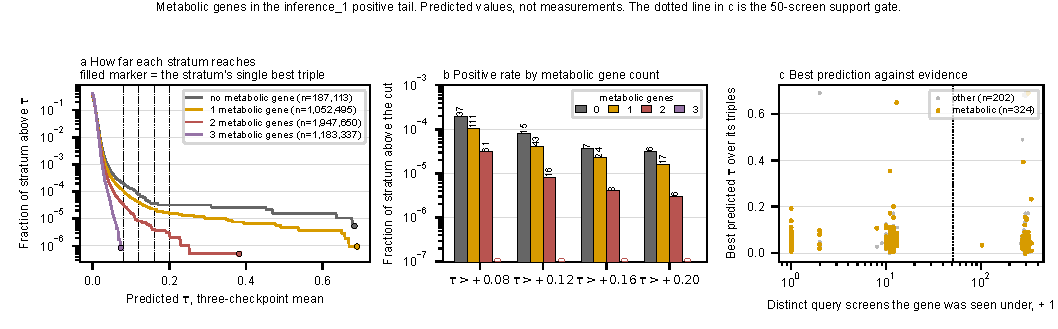
\includegraphics[width=\linewidth]{figures/metabolic_positive_predictions.pdf}
\caption{How far each metabolic stratum reaches into the positive tail, the
positive rate at each cut with counts labeled including the zeros, and each
gene's best prediction against the number of distinct query screens it was seen
under. Generated by
\protect\file{experiments/010-kuzmin-tmi/scripts/metabolic\_positive\_predictions.py}.}
\end{figure}
